\section{\Large PROBLEM SET 1}
\subsection{PROBLEM 1}
\textit{Select some key ADCS characteristics of your mission, including orbit (e.g., LEO, MEO, GEO, HEO, Interplanetary), target attitude (e.g., Sun pointing, Inertial pointing, Earth pointing, Resident Space Object pointing), attitude state representation (e.g., Euler angles, Gibbs vector, Quaternions Direction Cosine Matrix, Euler Axis/Angle), sensors suite (Gyros, Magnetometers, Star Trackers, Earth Sensor, Sun Sensor), actuator suite (Thrusters, Magnetorquers, Reaction Wheels, Momentum Wheel, Gravity Gradient).}

The ultimate goal of the project is to work on a satellite using synthetic aperture radar (SAR) designed to gather key environmental data on Earth. The satellite will be in low Earth orbit (LEO) and a state described in quaternoins to avoid gimble locking. For state estimation, the spacecraft will require gyroscopes, star trackers, and a potentially a sun sensor. For actuation, the spacecraft will likely require thrusters, reaction wheels, and magnetorquers.

\subsection{PROBLEM 2}
\textit{Conduct survey of satellites which have characteristics similar to selected project. Use internet, publications, and books as resources.}

Space agencies such as NASA have had a vested interest in being able to gather satellite images and data from Earth for decades now. Because of this, many satellites have been designed to do what we aim to do.

For example, Soil Moisture Active Passive (SMAP) is a NASA satellite launched in 2015 that utilizes L-band synthetic aperture radar (SAR) technology to measure soil moisture from LEO. This data has applications in climate change research climate change research applications (such as updating climate models) and some day-to-day activities (such as improving weather forecasts). SMAP was unique in the sense that it had a large deployable reflector that was attached to a boom \cite{SMAP}. In addition, the companies EOSSAR and Capella Space are developing satellites that use SAR technology in the X-band and S-band regimes for applications ranging from agriculture to mining \cite{EOSSAR, Capella}. Additionally, agencies have been partnering up to create SAR satellites. The most notable example is NASA and ISRO partnering to work on NASA-ISRO Synthetic Aperture Radar (NISAR), which is a satellite that captures data in the L-band and S-band SAR frequencies \cite{NisarMission}. Overall, the unique capabilities of NISAR over the other satellites and the availability of data for it made NISAR the prime candidate for this project.

\subsection{PROBLEM 3}
\textit{Select preferred existing satellite and payload for project. Similarity is helpful, but not strictly required.}

We select the NASA JPL and ISRO NISAR mission as the mission on which to base our satellite. Later, we will simplify some of the geometries for our analysis.

\subsection{PROBLEM 4}
\textit{Collect basic information on mission, requirements, ADCS sensors and actuators, mechanical layout, mass, mass distribution, and inertia properties.}

NISAR is a joint earth-observation satellite missions between NASA and ISRO. It is the first satellite to use two different Synthetic Aperture Radar (SAR) technologies in both the L-band and S-band. Both frequencies can penetrate clouds, but the L-band can penetrate thicker vegetation that the S-band cannot. Meaning, NISAR has the unique ability to be used in far more applications than previous SAR satellites, ranging from disaster response to agriculture cases \cite{NisarApps}.



As shown in \textbf{Figure 1}, NISAR's satellite consists of a 1.9 m x 1.8 m x 1.2 m spacecraft bus cuboid with a 1.2 m wide octagonal Radar Instrument Structure (RIS). The satellite is powered by a 23 m$^2$ solar panel array split on the left and right side of the satellite. Additionally, a 12 m diameter radar antenna is held up by a 9 m long boom with a 7" x 7" cross-section area \cite{NisarMission}.

Table \ref{NisarMassProps} contains mass properties of the satellite. Unfortunately, mass distribution and inertia properties of NISAR are not publicly available, so they were omitted from the report. However, they are estimated in the next section.

\begin{table}
\caption{Mass properties of NISAR}
\centering
\begin{tabular}{|l|l|}
\hline
\textbf{Component}               & \textbf{Mass (kg)} \\ \hline
Radar Instrument Structure (RIS) & 1375.9             \\ \hline
Spacecraft Bus                   & 964.1              \\ \hline
Radar Antenna Boom (RAB)         & 192                \\ \hline
Radar Antenna Reflector (RAR)    & 100                \\ \hline
Solar Array (total)              & 46                 \\ \hline
Total                            & 2678               \\ \hline
\end{tabular}
\label{NisarMassProps}
\end{table}

Since NISAR is a relatively large satellite, it has a complex ADCS system with an array of sensors and actuators. Sensors include star sensors, sun sensors, GPS, and a 3-axis gyroscope for roll, pitch, and yaw. For actuators, NISAR has four 50 N$\cdot$m reaction wheels mounted tetrahedral, three 565 and 350 A$\cdot$m$^2$ magnetorquers, and fourteen thrusters (ten canted 11 N thrusters, one central 11 N thruster, and four 1 N thrusters for roll) \cite{NisarMission}.

\subsection{PROBLEM 5}
\textit{Simplify spacecraft geometry, make assumptions on mass distribution, e.g. splitting it in its core parts, define body axes (typically related to geometry and payload), compute moments of inertia and full inertia tensor w.r.t. body axes. Show your calculations.}

We simplify the spacecraft geometry into six components, each individually assumed to have uniform mass distribution. These components of the simplified geometry are: bus structure, RIS (Radar Instrument Structure), RAB (radar antenna boom), RAR (radar antenna reflector), and two solar panels (identified as the +y solar panel and -y solar panel). The bus structure is modeled as a rectangular prism, while the RIS is modeled as an octagonal prism. The RAB is also modeled as a rectangular prism, while the RAR is modeled as a thin disk and the solar panels are modeled as thin rectangular plates. Within each geometry, our model assumes mass is distributed uniformly. From analyzing diagrams found in technical reports, we estimate that the RAR is tilted -3.87\degree about the y-axis (relative to the x-axis), while the RAB is modeled as a single beam with an angle approximately -18\degree from vertical (from the z-axis, about the y-axis in the x-z plane).

\subsection{PROBLEM 6}
\textit{Discretize your spacecraft through its outer surfaces (geometry). Develop a Matlab/Simulink function to handle barycenter (geometry, no mass distribution) coordinates, size, and unit vectors normal to each outer surface of the spacecraft in body frame. You can list all this information in a Matrix. This will be essential later on to compute environmental torques acting on the spacecraft from forces, surface orientation, and the vectors connecting the satellite’s center of mass to each surface’s center of mass.}

For the purpose of discretizing the spacecraft into surfaces, we consider the outer faces of the bus, RIS, and RAB. We also consider the faces of the solar panels and RAR, which are modeled as thin plates. The centroid (barycenter) coordinates and area for each surface are obtained using the surface properties tool in SolidWorks, and a unit normal vector is manually computed based on the orientation of the surface. We then enter this data into a CSV file, which can be read into MATLAB using the following function:

\lstinputlisting{src/surfaces.m}

This function stores the data into arrays of barycenter coordinates, unit normal vector components, and area. Each row of an array corresponds to a particular surface. The data is shown in Table \ref{tab:surfaces}, annotated with the identity of each surfaces.

\begin{longtable}{lrrrrrrr}
\caption{Surface parameters}
\label{tab:surfaces}\\
 &
  \multicolumn{3}{c}{\textbf{Barycenter [m]}} &
  \multicolumn{3}{c}{\textbf{Normal}} &
  \multicolumn{1}{l}{} \\
\endfirsthead
%
\endhead
%
\textbf{Surface} &
  \multicolumn{1}{l}{\textbf{x}} &
  \multicolumn{1}{l}{\textbf{y}} &
  \multicolumn{1}{l}{\textbf{z}} &
  \multicolumn{1}{l}{\textbf{x}} &
  \multicolumn{1}{l}{\textbf{y}} &
  \multicolumn{1}{l}{\textbf{z}} &
  \multicolumn{1}{l}{\textbf{Area [m\textsuperscript{2}]}} \\
Bus front, minus RIS (+x) & 0.6   & 0     & 0     & 1      & 0      & 0      & 2.4   \\
Bus rear (-x)                  & -0.6  & 0     & 0     & -1     & 0      & 0      & 3.42  \\
Bus side (+y)                  & 0     & 0.9   & 0     & 0      & 1      & 0      & 2.28  \\
Bus side (-y)                  & 0     & -0.9  & 0     & 0      & -1     & 0      & 2.28  \\
Bus top (+z)                   & 0     & 0     & 0.95  & 0      & 0      & 1      & 2.16  \\
Bus bottom (-z)                & 0     & 0     & -0.95 & 0      & 0      & -1     & 2.16  \\
RIS front (+x)                 & 3.1   & 0     & 0     & 1      & 0      & 0      & 1.02  \\
RIS top (+z)                   & 1.85  & 0     & 0.55  & 0      & 0      & 1      & 1.15  \\
RIS bottom (-z)                & 1.85  & 0     & -0.55 & 0      & 0      & -1     & 1.15  \\
RIS side (+y)                  & 1.85  & 0.55  & 0     & 0      & 1      & 0      & 1.15  \\
RIS side (-y)                  & 1.85  & -0.55 & 0     & 0      & -1     & 0      & 1.15  \\
RIS angle face (y-z I)         & 1.85  & 0.39  & 0.39  & 0      & 0.707  & 0.707  & 1.15  \\
RIS angle face (y-z II)        & 1.85  & -0.39 & 0.39  & 0      & -0.707 & 0.707  & 1.15  \\
RIS angle face (y-z III)       & 1.85  & -0.39 & -0.39 & 0      & -0.707 & -0.707 & 1.15  \\
RIS angle face (y-z IV)        & 1.85  & 0.39  & -0.39 & 0      & 0.707  & -0.707 & 1.15  \\
Panel +y front (+x)            & 0     & 3.9   & 0     & 1      & 0      & 0      & 11.4  \\
Panel +y rear (-x)             & 0     & 3.9   & 0     & -1     & 0      & 0      & 11.4  \\
Panel -y front (+x)            & 0     & -3.9  & 0     & 1      & 0      & 0      & 11.4  \\
Panel -y rear (-x)             & 0     & -3.9  & 0     & -1     & 0      & 0      & 11.4  \\
RAB front (x-z, +x)            & -0.81 & 0     & 5.21  & 0.951  & 0      & 0.309  & 1.6   \\
RAB rear (x-z, -x)             & -0.99 & 0     & 5.18  & -0.951 & 0      & -0.309 & 1.6   \\
RAB side (+y)                  & -0.9  & -0.09 & 5.19  & 0      & 1      & 0      & 1.6   \\
RAB side (-y)                  & -0.9  & 0.09  & 5.19  & 0      & -1     & 0      & 1.6   \\
RAB top (+z)                   & -2.31 & 0     & 9.47  & 0      & 0      & 1      & 0.03  \\
RAR top (+z)                   & 4.28  & 0     & 8.31  & -0.067 & 0      & 0.998  & 113.1 \\
RAR bottom (-z)                & 4.28  & 0     & 8.31  & 0.067  & 0      & -0.998 & 113.1
\end{longtable}

\subsection{PROBLEM 7}
\textit{At this stage you should have a simple 3D model of your spacecraft including geometry and mass properties of each element. Plot body axes (triad) in 3D superimposed to spacecraft 3D model.}

A 3D model of the spacecraft is shown in [FIGURE]. The body axes are shown, where the origin is chosen as the center of the spacecraft bus.

\begin{figure}[H]
\centering
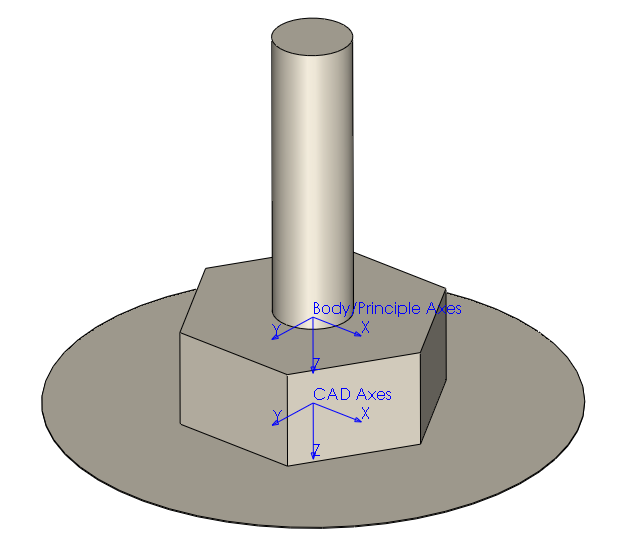
\includegraphics[scale=0.7]{Images/WMAP_CAD4.PNG}
\caption{A 3D model of the simplified satellite geometry. The body and principal axes are labeled and located at the spacecraft center of mass.}
\label{CAD model with frames}
\end{figure}


\begin{equation}
\vec{M} = \vec{I} \cdot \vec{\dot{\omega}}\ + \vec{\omega} \times \vec{I} \cdot \vec{\omega} \\ 
\end{equation}   

\begin{eqnarray}
M_x = I_{xx} \dot{\omega_x} + (I_{zz} - I_{yy})\omega_y \omega_z \nonumber \\
M_y = I_{yy} \dot{\omega_y} + (I_{xx} - I_{zz})\omega_z \omega_x \\
M_z = I_{zz} \dot{\omega_z} + (I_{yy} - I_{xx})\omega_x \omega_y \nonumber
\end{eqnarray}

\begin{equation}
I_{B} =
\begin{bmatrix} 
I_{xx} & I_{xy} & I_{xz} \\
I_{yx} & I_{yy} & I_{yz} \\ 
I_{zx} & I_{zy} & I_{zz} \\
\end{bmatrix}
=
\begin{bmatrix}
1005.5 & 0 & 0 \\
0 & 1005.5 & 0 \\ 
0 & 0 & 543.7
\end{bmatrix}
[kg/m^2].
\end{equation}

\begin{lstlisting}
function L_loc = LagrangePoints(mu)
%For a given value of mu, this function computes the location
%of all five Lagrange points for the circular restricted three
%body problem.

%Compute the location of the libration points
    l = 1 - mu;

    L_loc = zeros(5,3);

    %L1
    p_L1 = [1, 2*(mu - l), l^2 - 4*l*mu + mu^2, 2*mu*l*(l - mu) + mu - l,...
        mu^2*l^2 + 2*(l^2 + mu^2), mu^3 - l^3];
    L1roots = roots(p_L1);
    L1 = 0;
    for i = 1:5
        if (L1roots(i) > -mu) & (L1roots(i) < l)
         L1 = L1roots(i);
        end
    end
    L_loc(1,1) = L1;

    %L2
    %L3
    %L4
    %L5
end
\end{lstlisting}